\documentclass[a4paper]{article}
\usepackage[utf8]{inputenc}
\usepackage[T1]{fontenc}
\usepackage{lmodern}
\usepackage{listings}
\usepackage{graphicx}
\usepackage{dirtree}
\usepackage{caption}
\usepackage{subcaption}
\usepackage{float}
\usepackage[english]{babel}
\usepackage[margin=1.1in]{geometry}
\title{Localizer User Manual}
\author{\textsc{SIPP Florian}}
\lstset{
	frame = single,
	basicstyle = \footnotesize\ttfamily
}

\begin{document}
\maketitle
\begin{abstract}
This document is the user manual of the Software Localizer. Localizer is being developed by the Centre de Recherche en Neurosciences de Lyon (CRNL) to allow the quick analysis of data recovered during Localizer tasks performed by iEEG patients before their possible surgery due to drug resistant epilepsy.  Localizer is also the term used to define a set of tasks requiring the use of specific cognitive abilities. Those tasks will allow the researcher or the clinician to check for indications of epileptic activity in specific areas of the brain. 
\end{abstract}
\tableofcontents
\section{Data Curation} \label{curation}    
\paragraph{} In order to get the most of Localizer you need to organise your data in a specific way => 
\begin{figure}[H]
\framebox[\textwidth]{%
\begin{minipage}{0.9\textwidth}
\dirtree{%
	.1 HOSPITAL{\_}YEAR{\_}PATID/.
	.2 HOSPITAL{\_}YEAR{\_}PATID{\_}TASK1/.
	.3 HOSPITAL{\_}YEAR{\_}PATID{\_}TASK1.TRC.
	.3 ....
	.2 HOSPITAL{\_}YEAR{\_}PATID{\_}TASK2/.
	.3 HOSPITAL{\_}YEAR{\_}PATID{\_}TASK2.TRC.
	.3 ....
	.2 HOSPITAL{\_}YEAR{\_}PATID{\_}TASK3/.
	.3 HOSPITAL{\_}YEAR{\_}PATID{\_}TASK3.TRC.
}
\end{minipage}
}
\caption{\label{projectDirectory}Project directory hierarchy}
\end{figure}

\section{Options} \label{options}    
\subsection{Localizer}
\paragraph{} This option menu will let you create .prov files. The .prov extension stands for \textbf{protocol visualization}. Typically, a Localizer is a set of time series (one for each channel) with data for each sample from the beginning to the end of the recording session. In addition,  information about the events of the experimental paradigm is stored, each event being identified using a code (e.g. an event of code 10 occured at sample 134567).
\paragraph{} The .prov file instructs Localizer on how to epoch the data based on the events. It consists of blocs which contain a list of subblocs. Each bloc or subbloc will be sorted using first their respective order and then alphabetically using their respective names.
\paragraph{} Each subbloc is centered around a specific event, called \textbf{main event}, for a specific time window (for instance, consider all events with code 10 and extract for each of them a window ranging from 200ms before to 700ms after that event). You can specify secondary events which do not interfere in the epoching. You can also set a baseline window, which is used for statistical analysis.
\paragraph{} Each bloc also has a sorting method, which is used to sort the trials obtained from the epoching according to specific conditions (code of the main event, latency of the secondary event...). The syntax used here for a condition is \textit{SUBBLOC{\_}EVENT{\_}COMMAND} where SUBBLOC is the name of the sub-bloc, EVENT the name of the event and COMMAND the sorting parameter (which can be LATENCY or CODE). You can specify multiple conditions which are separated by a semi-colon, each of which are interpreted in the order they have been written. The rest of the .prov file is straightforward: you can specify images (.png or .jpg) at specific time windows, or to associate an image to a bloc. 
\subsection{File Priority}
\subsection{Statistic}
\subsection{Pictures}
\subsection{Frequency Bands}

\section{Data Analysis} \label{analysis}    
\subsection{Hilbert Transform}
\paragraph{} The signal for each contact was first bandpass‐filtered in multiple successive 10 Hz wide frequency bands (e.g. 10 bands from [50–60 Hz] to [140–150 Hz]) using a zero phase shift no causal finite impulse filter with 0.5 Hz roll‐off. The envelope of each bandpass‐filtered signal was then computed with a standard Hilbert transform then down‐sampled to 64 Hz and divided by its means across the entire recording session and multiplied by 100, to express each value as a percentage of that mean (normalization).  

\begin{figure}[H]
\begin{center}
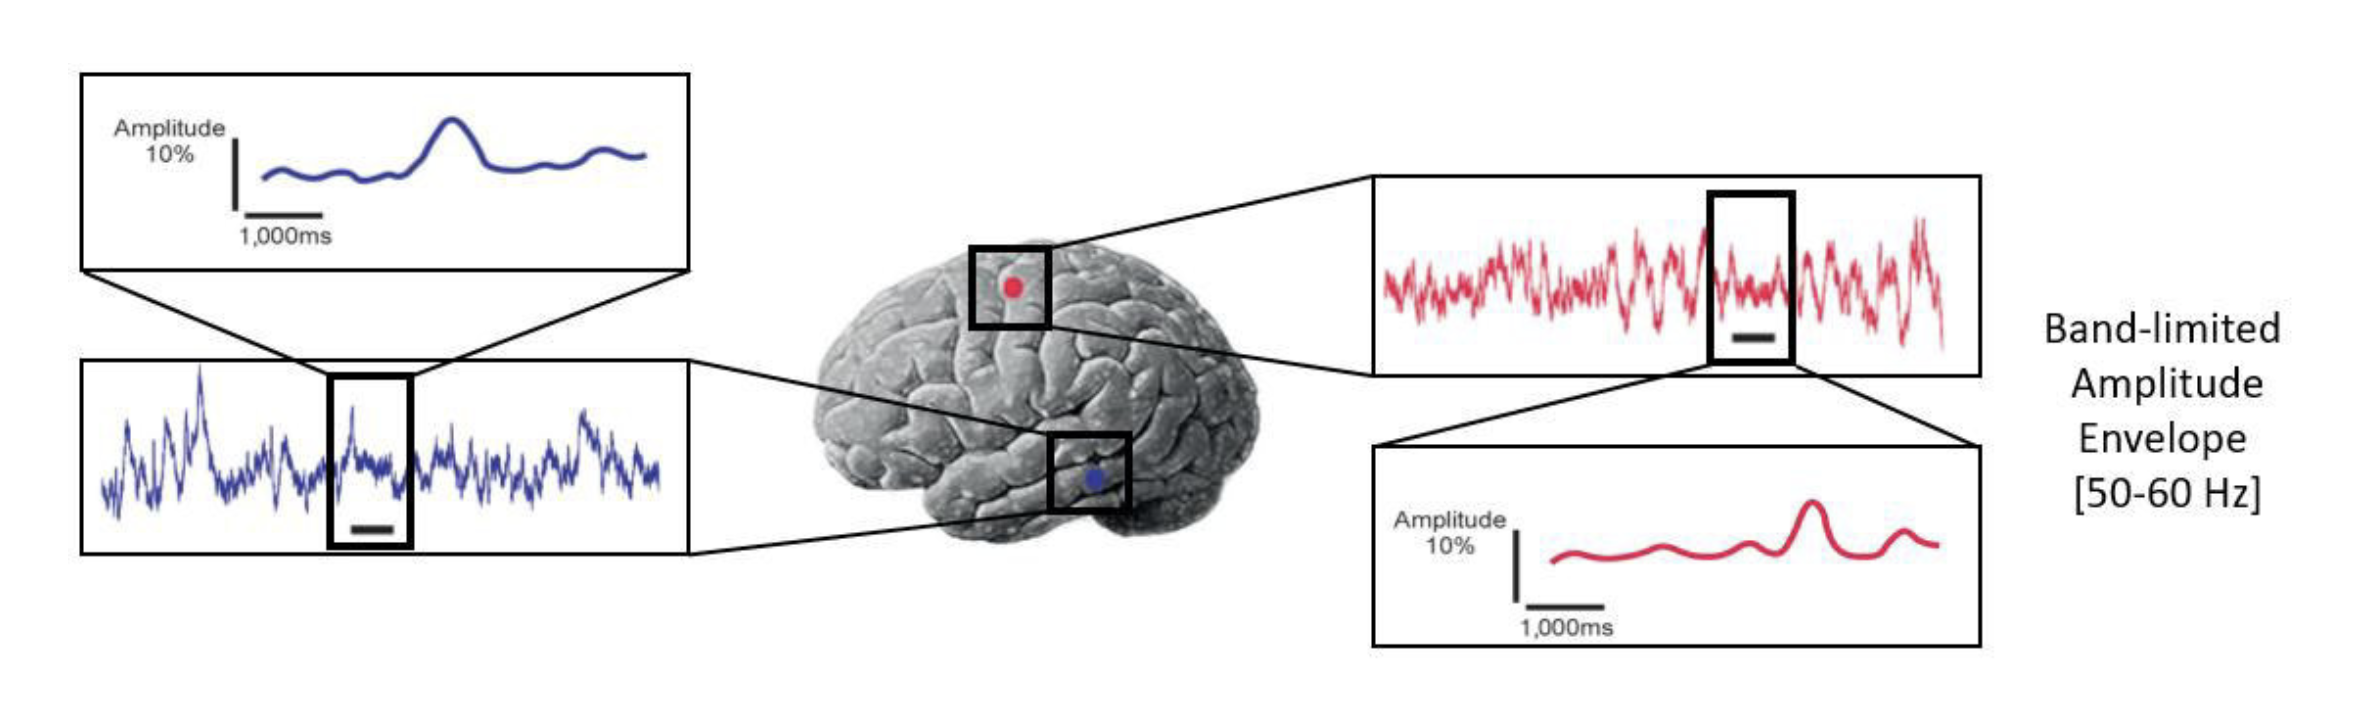
\includegraphics[scale=0.4]{HilbertProcessing.png}
\end{center}
\caption{\label{HilbertProcessingPicture}Hilbert Transform of raw IEEG Data}
\end{figure}

Finally, the normalized envelope signals for each of the ten frequency band were averaged together to provide a single HFA signal. By construction, the mean value of that HFA signal across the entire recording session is equal to 100. The whole procedure is also designed to reduce the 1/f drop‐off in amplitude of the raw iEEG signals. 

\subsection{Envelope Plot}
\paragraph{} Still blabla
\begin{figure}[H]
\begin{center}
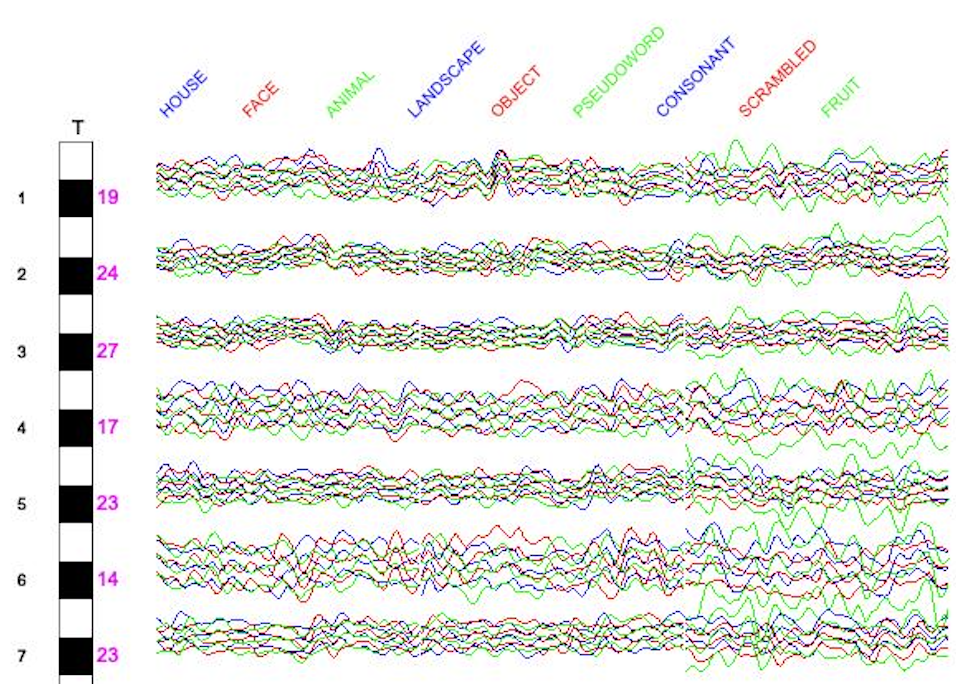
\includegraphics[scale=0.8]{EnvelopePlots.png}
\end{center}
\caption{\label{EnvelopePlotsPicture}Gamma Band activity for each contact and each conditions during the visual task}
\end{figure}
\subsection{Time Trials Matrices}
\paragraph{} Still blabla
\begin{figure}[H]
\begin{center}
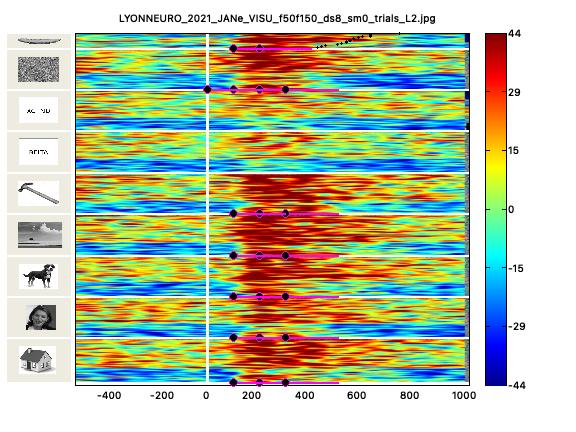
\includegraphics[scale=0.7]{TimeTrialsMatrice.jpg}
\end{center}
\caption{\label{TimeTrialsPicture}Gamma Band activity during the visual task}
\end{figure}
\subsection{Correlation Maps}
\paragraph{} Still blabla
\subsection{Statistical Files}
\paragraph{} Still blabla
\end{document}